\section{Tracking-by-Assignment}
\label{sec:tracking-by-assignment}

A common cell tracking approach is dividing the procedure into two phases, namely
\begin{enumerate}
      \item the \emph{detection} or \emph{segmentation} phase, followed by
      \item the \emph{assignment} or \emph{tracking} phase.
\end{enumerate}
Its strengths are the ability to handle false positive detections and cope with an unknown number of
cells as well as dividing targets.  A possible tracking-by-assignment pipeline is depicted in
\cref{fig:cg-hypotheses}: For each time step the detection algorithm produces a set of cell
candidates that are likely to be -- but not necessarily are -- actual cells. During the tracking
phase, candidates of consecutive time steps are brought into relation to each other by creating
\emph{assignment hypotheses}. Out of these hypotheses the tracking algorithm chooses that set of
assignments that is optimal, \ie the one which best describes the motion of all cells over all
time steps.
% It is the tracking algoritm's task to define constraints on valid sets of
% assignments as well as a method for determining the optimal solution.
A simple example of a tracking-by-assignment algorithm is the ``nearest neighbor tracker'', that
greedily assigns to a cell at time $t$ its nearest neighbor at time $t+1$. It is obvious that,
especially in dense cell populations, this approach is likely to produce an optimal solution that is
far from the actual cell movement in the raw data. More robust tracking-by-assignment methods are
the \emph{chain graph} (\cref{subsec:fg-chaingraph}) or \emph{conservation} tracking
(\cref{subsec:fg-conservation}).  An approach that -- while being inspired by tracking-by-assignment
-- breaks the fixed border between detection and tracking is introduced in \cref{cha:joint} as the
\emph{joint segmentation and tracking} and is the main contribution of this thesis.

After a brief introduction of the hypotheses graph in \cref{subsec:hypotheses-graph},
\cref{sec:tracking-as-a-factor-graph} utilizes the power of graphical models
(\cref{sec:gm-graphical-models}) for approaching the tracking challenge.

\begin{figure}
    \centering
    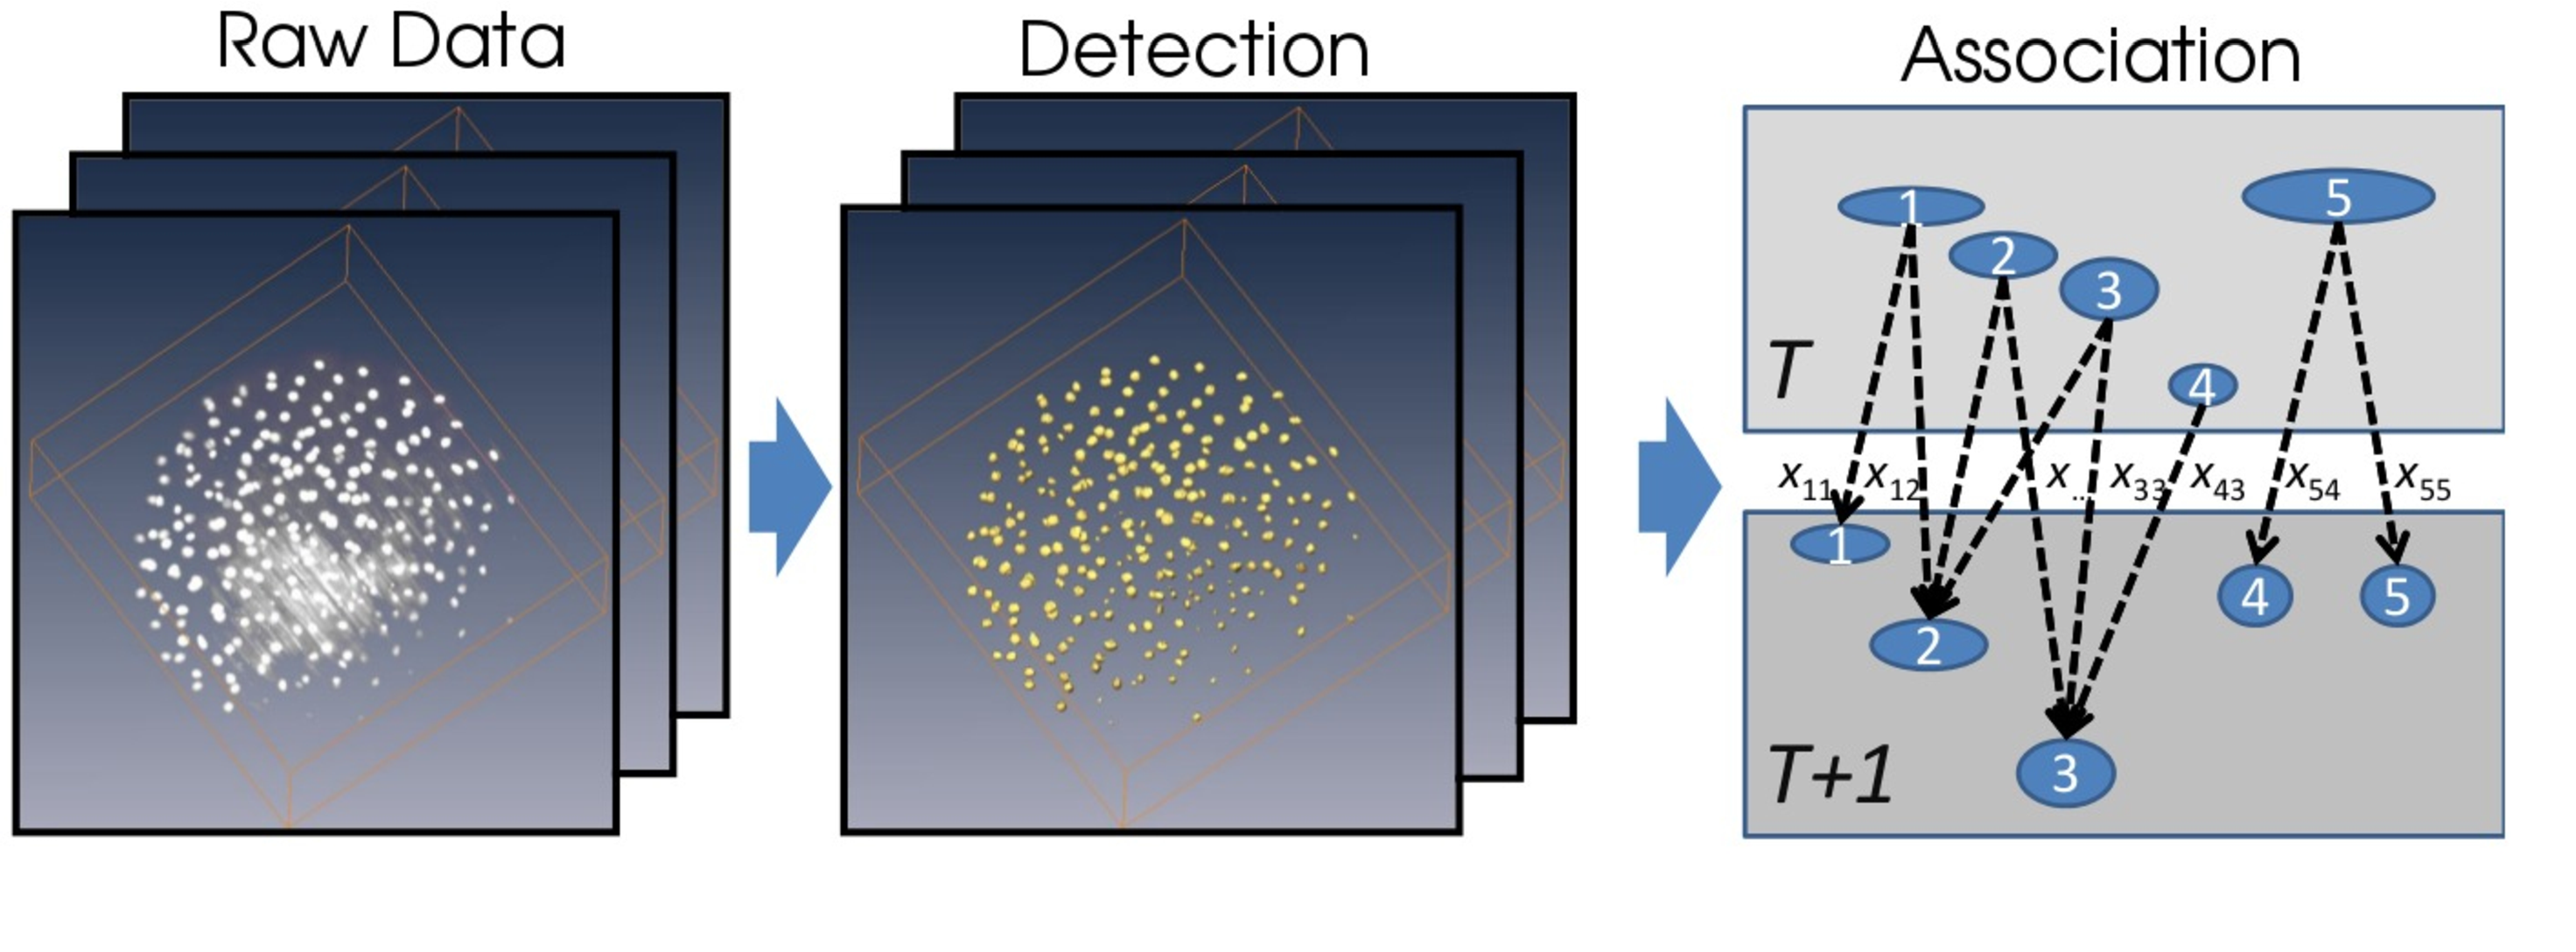
\includegraphics[width=\textwidth]{images/chaingraph/pipeline.pdf}
    %\rule{\textwidth}{0.3pt}
    \caption[Tracking-by-assignment pipeline]{Tracking-by-assignment pipeline, taken from
        \citet[9]{kausler_13_tracking}. Cell candidates are extracted from raw data by
        segmentation. Possible assignments (associations) are subsumed in the \emph{hypotheses
            graph}, as introduced by \citet[Chapter~3.1]{kausler_13_tracking}. The
        hypotheses graph does not describe a valid tracking (\eg cell $3$ in time step $T+1$ would
        have three parents), but a valid and optimal subset of the hypotheses can be concluded. Note
        that here assignment variables are described by $X_{ij}$. Throughout this thesis, variables
        named $X$ refer to detections, while assignments are referred to as $Y$.}
    \label{fig:cg-hypotheses}
\end{figure}


\subsection{Hypotheses Graph}
\newsavebox{\captionHypotheses}
\savebox{\captionHypotheses}{\small\tikz[baseline, inner
    sep=1pt]\node[thick, draw, circle, color=black, text=black] at (0,2.5pt){\tiny $X$};}

\label{subsec:hypotheses-graph}
The \emph{hypotheses graph} \citep[Chapter~3.1]{kausler_13_tracking} is a graphical
representation of possible assignments between cell detections. In general, any hypothetical
assignment between two cells is possible. However, in order to reduce the problem size, assignments
are restricted to cells in consecutive time steps. Moreover, only the $k$ nearest neighbors within a
thresholded distance at time step $t+1$ of a cell at time step $t$ are valid candidates for
assignment hypotheses, where $k$ is a design parameter of the model. In the graphical representation
of a toy example in \cref{fig:tba-hypotheses-graph} detections are depicted by nodes
({\protect\usebox{\captionHypotheses}}), while edges denote assignments. Note that, in general, the
position of the nodes in the hypotheses graph does not reflect the position of the corresponding
detections in raw data.

The tracking model is formulated as an algorithm that incorporates constraints and a quality measure
for feasible solutions in order to find the optimal tracking result. In the tracking models that are
discussed in this thesis (\cref{subsec:fg-chaingraph,subsec:fg-conservation,cha:joint}), these
constraints and measures are implemented in terms of a probabilistic graphical model.


\begin{figure}
    \centering
    \begin{subfigure}{0.44\textwidth}
        \centering
        \scalebox{0.9}{
            \begin{tikzpicture}[minimum size=58pt,scale=0.45, every node/.style={scale=0.45, text=black, font=\LARGE}, thick]
                    \begin{scope}
        \node (t1) {\huge $t$};
        \node[hypothesesdetection, below=of t1, circle, draw] (x11) {$X_1^t$};
        \node[hypothesesdetection, below=of x11, circle, draw] (x12) {$X_2^t$};
        \node[hypothesesdetection, below=of x12, circle, draw] (x13) {$X_3^t$};
    \end{scope}

    
    
    \begin{scope}
        \node[right=of t1, xshift=15mm] (t2) {\huge $t+1$};
        \node[hypothesesdetection, below=of t2, circle, draw] (x21) {$X_4^{t+1}$};
        \node[hypothesesdetection, below=of x21, circle, draw] (x22) {$X_5^{t+1}$};
    \end{scope}

    \begin{scope}[on background layer]
        \node[hypothesesdetection, below=of x22, circle, draw, on background layer] (x23) {$X_6^{t+1}$};
    \end{scope}
    
    
    \begin{scope}
        \node[right=of t2, xshift=15mm] (t3) {\huge $t+2$};
        \node[hypothesesdetection, below=of t3, circle, draw] (x31) {$X_7^{t+2}$};
        \node[hypothesesdetection, circle, draw, shift=($(x31.center)-(x21.center)$)] (x32) at (x22) {$X_8^{t+2}$};
    \end{scope}
    
    \begin{scope}[on background layer]
        \node[hypothesesdetection, below=of x32, circle, draw, on background layer] (x33) {$X_{10}^{t+2}$};
    \end{scope}
    
    % \begin{scope}
    %     \node[right=of t3, xshift=15mm] (t4) {\huge $t+3$};
    %     \node[hypothesesdetection, below=of t4, circle, draw] (x41) {$X_{10}^{t+3}$};
    %     \node[hypothesesdetection, below=of x41, circle, draw] (x42) {$X_{11}^{t+3}$};
    %     \node[hypothesesdetection, below=of x42, circle, draw] (x43) {$X_{12}^{t+3}$};
    % \end{scope}

    \begin{scope}[on background layer]
        \node[rectangle, draw, color=hypothesesbackground!40, fill=hypothesesbackground!30,
        fit=(x11) (x12) (x13), inner sep=13mm] (b1) {};
        \node[rectangle, draw, color=hypothesesbackground!40, fill=hypothesesbackground!30,
        fit=(x21) (x22) (x23), inner sep=13mm] (b2) {};
        \node[rectangle, draw, color=hypothesesbackground!40, fill=hypothesesbackground!30,
        fit=(b2), shift=($(t3.center) - (t2.center)$), inner sep=-0.1mm] (b3) {};
        % \node[rectangle, draw, color=hypothesesbackground!40, fill=hypothesesbackground!30,
        % fit=(x41) (x42) (x43), inner sep=13mm] (b4) {};
    \end{scope}

    \path[hypothesestransition] (x11) edge (x21);
    \path[hypothesestransition] (x12) edge (x22);
    \path[hypothesestransition] (x13) edge (x22);
    % \path[hypothesestransition] (x13) edge (x23);

    \path[hypothesestransition] (x21) edge (x31);
    \path[hypothesestransition] (x21) edge (x32);
    \path[hypothesestransition] (x22) edge (x32);
    % \path[hypothesestransition] (x23) edge (x32);

    % \path[hypothesestransition] (x31) edge (x41);
    % \path[hypothesestransition] (x32) edge (x42);
    % \path[hypothesestransition] (x32) edge (x43);

%%% Local Variables: 
%%% mode: latex
%%% TeX-master: "../../../main"
%%% End: 



%%% Local Variables: 
%%% mode: latex
%%% TeX-master: "../../main"
%%% End: 

            \end{tikzpicture}
        }
        \caption{Hypotheses Graph}
        \label{subfig:hypotheses-graph-example}
    \end{subfigure}
    \hfill
    \begin{subfigure}{0.44\textwidth}
        \centering
        \scalebox{0.9}{
            \begin{tikzpicture}[minimum size=58pt,scale=0.45, every node/.style={scale=0.45, text=black, font=\LARGE}, thick]
                    \begin{scope}
        \node (t1) {\huge $t$};
        \node[hypothesesdetection, below=of t1, circle, draw] (x11) {$X_1^t$};
    \end{scope}
    \begin{scope}[on background layer]
        \node[hypothesesdetection, below=of x11, circle, draw] (x12) {$X_2^t$};
    \end{scope}
    \begin{scope}
        \node[hypothesesdetection, below=of x12, circle, draw] (x13) {$X_3^t$};
    \end{scope}

    
    
    \begin{scope}
        \node[right=of t1, xshift=15mm] (t2) {\huge $t+1$};
        \node[hypothesesdetection, below=of t2, circle, draw] (x21) {$X_4^{t+1}$};
        \node[hypothesesdetection, below=of x21, circle, draw] (x22) {$X_5^{t+1}$};
    \end{scope}

    \begin{scope}[on background layer]
        \node[hypothesesdetection, below=of x22, circle, draw, on background layer] (x23) {$X_6^{t+1}$};
    \end{scope}
    
    
    \begin{scope}
        \node[right=of t2, xshift=15mm] (t3) {\huge $t+2$};
        \node[hypothesesdetection, below=of t3, circle, draw] (x31) {$X_7^{t+2}$};
        \node[hypothesesdetection, circle, draw, shift=($(x31.center)-(x21.center)$)] (x32) at (x22) {$X_8^{t+2}$};
    \end{scope}
    
    \begin{scope}[on background layer]
        \node[hypothesesdetection, below=of x32, circle, draw, on background layer] (x33) {$X_{10}^{t+2}$};
    \end{scope}
    
    % \begin{scope}
    %     \node[right=of t3, xshift=15mm] (t4) {\huge $t+3$};
    %     \node[hypothesesdetection, below=of t4, circle, draw] (x41) {$X_{10}^{t+3}$};
    %     \node[hypothesesdetection, below=of x41, circle, draw] (x42) {$X_{11}^{t+3}$};
    %     \node[hypothesesdetection, below=of x42, circle, draw] (x43) {$X_{12}^{t+3}$};
    % \end{scope}

    \begin{scope}[on background layer]
        \node[rectangle, draw, color=hypothesesbackground!40, fill=hypothesesbackground!30,
        fit=(x11) (x12) (x13), inner sep=13mm] (b1) {};
        \node[rectangle, draw, color=hypothesesbackground!40, fill=hypothesesbackground!30,
        fit=(x21) (x22) (x23), inner sep=13mm] (b2) {};
        \node[rectangle, draw, color=hypothesesbackground!40, fill=hypothesesbackground!30,
        fit=(b2), shift=($(t3.center) - (t2.center)$), inner sep=-0.1mm] (b3) {};
        % \node[rectangle, draw, color=hypothesesbackground!40, fill=hypothesesbackground!30,
        % fit=(x41) (x42) (x43), inner sep=13mm] (b4) {};
    \end{scope}

    \path[hypothesestransition] (x11) edge (x21);
    % \path[hypothesestransition] (x12) edge (x22);
    \path[hypothesestransition] (x13) edge (x22);
    % \path[hypothesestransition] (x13) edge (x23);

    \path[hypothesestransition] (x21) edge (x31);
    % \path[hypothesestransition] (x21) edge (x32);
    \path[hypothesestransition] (x22) edge (x32);
    % \path[hypothesestransition] (x23) edge (x32);

    % \path[hypothesestransition] (x31) edge (x41);
    % \path[hypothesestransition] (x32) edge (x42);
    % \path[hypothesestransition] (x32) edge (x43);

%%% Local Variables: 
%%% mode: latex
%%% TeX-master: "../../../main"
%%% End: 



%%% Local Variables: 
%%% mode: latex
%%% TeX-master: "../../main"
%%% End: 

            \end{tikzpicture}
        }
        \caption{Possible tracking result}
        \label{subfig:hypotheses-graph-example-inferred}
    \end{subfigure}
    \caption[Exemplary hypotheses graph]{Exemplary hypotheses graph
        (\subref{subfig:hypotheses-graph-example}) with a potential, meaningful tracking result
        (\subref{subfig:hypotheses-graph-example-inferred}). Detections are represented by black
        circles, edges show assignment hypotheses. False positive detections and hypotheses are
        removed from the hypotheses graph after inference. The tracker decided, that $X_2^t$ was a
        false detection and corrected that error.}
    \label{fig:tba-hypotheses-graph}
\end{figure}

% $\protect\usebox{\captionTest}$,

%%% Local Variables: 
%%% mode: latex
%%% TeX-master: "../../main"
%%% End: 
